%%%%% Beginning of preamble %%%%%
\documentclass[12pt]{article} 

%What kind of document (article) and what size
%Packages to load which give you useful commands
\usepackage{amssymb, amsmath, amsthm} 
\usepackage{epsfig,graphicx} 
\usepackage{caption}
\usepackage{subcaption}


%Sets the margins
\textwidth = 6.5 in 
\textheight = 9 in 
\oddsidemargin = 0.0 in 
\evensidemargin = 0.0 in 
\topmargin = 0.0 in 
\headheight = 0.0 in 
\headsep = 0.0 in \parskip = 0.2in \parindent = 0.0in

\begin{document} 

\section{Network and Dynamics}

Before proceeding, we fix some notation, following \cite{kolaczyk2009statistical}. Let $G = (V, E)$ be the graph that represents the $|V|$ vertices in the network and the $|E|$ edges between them. We will consider a random field evolving in time on this network. That is, for a finite network, let $X(t, v)$ denote the random variable in some countable alphabet $\mathcal{X}_{v}$ associated with vertex $v$ at time $t$. Overall, $X(t, v)$ is a time-varying random field whose dynamics take place on $G$ and are effected by the topology of $G$. Thus, for fixed $t$, $X(t, \cdot)$ is a random vector and for fixed $v$, $X(\cdot, v)$ is a random field. We will occasionally refer to the random field at a fixed timepoint $t$ as $\mathbf{X}(t) = (X(t, v_{1}), \ldots, X(t, v_{|V|})).$

For the particular problem we consider here, $G$ corresponds to an (explicit) social network, and $X(t,v)$ corresponds to some observed behavior of an individual $v$ at time $t$.

\section{Edge Weighting using Dynamics}

\textbf{Put a brief rationale for why we use this approach.}

Let $X^{u} = X(\cdot, u).$ That is, in what follows we implicitly assume the stationarity of $X(t, v)$ with respect to time. Denoting the joint distribution of $(X^{u}, X^{v})$ as $p(x^{u}, x^{v})$ and the associated marginals as $p(x^{u})$ and $p(x^{v})$, we then define the mutual information between two individuals in the usual way~\cite{cover1994elements} as
\begin{align}
	I[X^{u}; X^{v}] &= E\left[\log_{2} \frac{p(X^{u}, X^{v})}{p(X^{u})p(X^{v})}\right]\\
	&= \sum_{x^{u} \in \mathcal{X}^{u}, x^{v} \in \mathcal{X}^{v}} p(x^{u}, x^{v}) \log_{2} \frac{p(x^{u}, x^{v})}{p(x^{u}) p(x^{v})}.
\end{align}
The mutual information is not generally bounded on a standard interval. To allow for standardized weightings, we follow~\cite{shalizi2007discovering} and normalize the mutual information, noting that
\begin{align}
	I[X^{u}; X^{v}] = H[X^{u}] - H[X^{u} | X^{v}] \leq H[X^{u}]
\end{align}
(by the positivity of $H[X^{u} | X^{v}]$), and equivalently
\begin{align}
	I[X^{u}; X^{v}] = H[X^{u}] - H[X^{u} | X^{v}] \leq H[X^{v}].
\end{align}
Overall, this implies that
\begin{align}
	I[X^{u}; X^{v}] \leq \min \left\{ H[X^{u}], H[X^{v}]\right\},
\end{align}
so dividing by $\min \left\{ H[X^{u}], H[X^{v}]\right\}$ gives the normalized mutual information
\begin{align}
	I^{*}[X^{u}; X^{v}] = \frac{I[X^{u}; X^{v}]}{\min \{ H[X^{u}], H[X^{v}]\}} \label{normalized-MI}
\end{align}
which lies between 0 and 1.

Of course, in an empirical study, we do not know the information theoretic quantities associated with any two users. Instead, we must infer them from an observed time series. To do so, we use the maximum likelihood estimates for all quantities~\cite{paninski2003estimation}. In the absence a parametric model (which we do not assume here), this amounts to using the plug-in estimator for $p(x^{u}, x^{v})$ in (\ref{normalized-MI}). Assuming we observe $\{ (X(t, u), X(t, v)) \}_{t = 1}^{T}$, the plug-in estimator for $p(x^{u}, x^{v})$ is simply
\begin{align}
	\hat{p}(x^{u}, x^{v}) = \frac{\#(X(t, u) = x^{u}, X(t, v) = x^{v})}{N},
\end{align}
the proportion of times we observe a particular behavior in both individuals out of all behaviors observed.

As observed in~\cite{paninski2003estimation}, all estimators for information theoretic quantities are biased, including the plug-in estimator. However, the bias is generally proportional to the size of the joint alphabet $\mathcal{X}^{u} \times \mathcal{X}^{v}$ and inversely proportional to the sample size $T$. Since we will typically take $\mathcal{X}^{u} = \{0, 1\}$ for all individuals $u$, $|\mathcal{X}^{u} \times \mathcal{X}^{v}| = 4$, and the bias will be small for the sample sizes we consider.

\section{Examples}

\subsection{Toy Model --- Coupled Bernoulli Processes Embedded in a Stochastic Block Model}

\textbf{Describe the toy model in generalities.}

\subsubsection{Stochastic Block Model}

We use the stochastic block model~\cite{holland1983stochastic} as a generative model for the structural network. The basic stochastic block model is a popular model for simple community structure. We will specify the community of a user $u$ by $C(u)$ and the set of all communities by $\mathcal{C}$. Each individual $u$ in the network is assigned to a (latent) community $C(u) = c \in \mathcal{C}$. Edges are then placed between each user $u$ and $v$ with probability $p_{uv} = p_{C(u), C(v)}$ depending only on the membership the two users. Typically, for assortative communities, $p_{cc} > p_{cc'}$ for all $c \neq c' \in \mathcal{C}$. That is, the density of links within a community is greater than the density of links between communities, which is the standard definition of community structure. If we fix $p_{cc} = p_{\text{in}}$ and $p_{cc'} = p_{\text{out}}$ for all $c \neq c' \in \mathcal{C}$, we obtain a weighting matrix like Figure \ref{Fig-SBM}. This clearly posses a `block' structure (hence the name stochastic block model) with clear communities. The adjacency matrix for a particular realization from this model resembles Figure \ref{Fig-SBM_Realization}.

\begin{figure}[h!]
  \centering
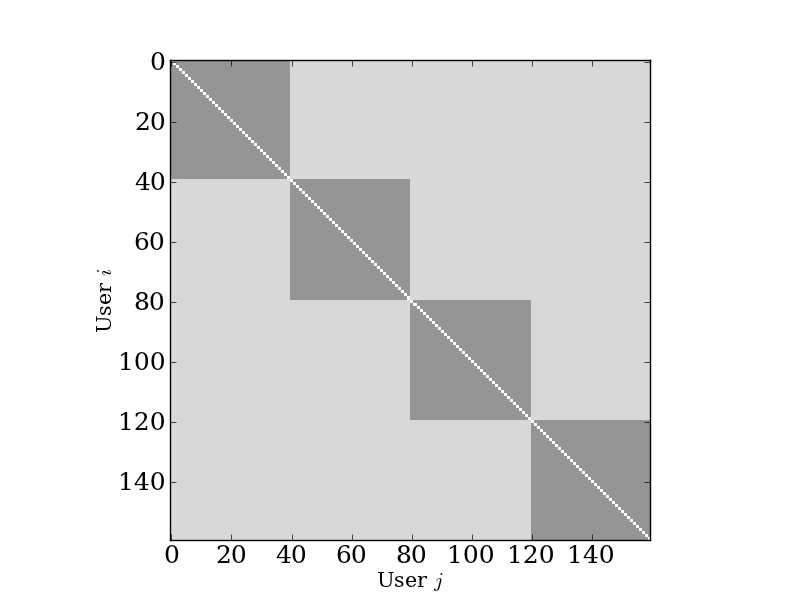
\includegraphics[width=0.75\textwidth]{Figures/prob_mat.png}
\caption{Lorem ipsum.}
\label{Fig-SBM}
\end{figure}

\begin{figure}[h!]
  \centering
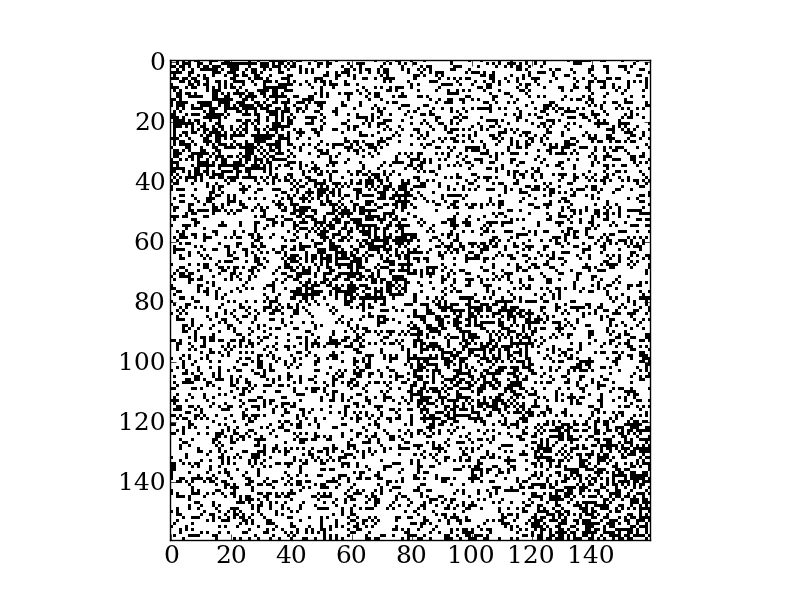
\includegraphics[width=0.75\textwidth]{Figures/adj_mat.png}
\caption{Lorem ipsum.}
\label{Fig-SBM_Realization}
\end{figure}

\begin{figure}[h!]
  \centering
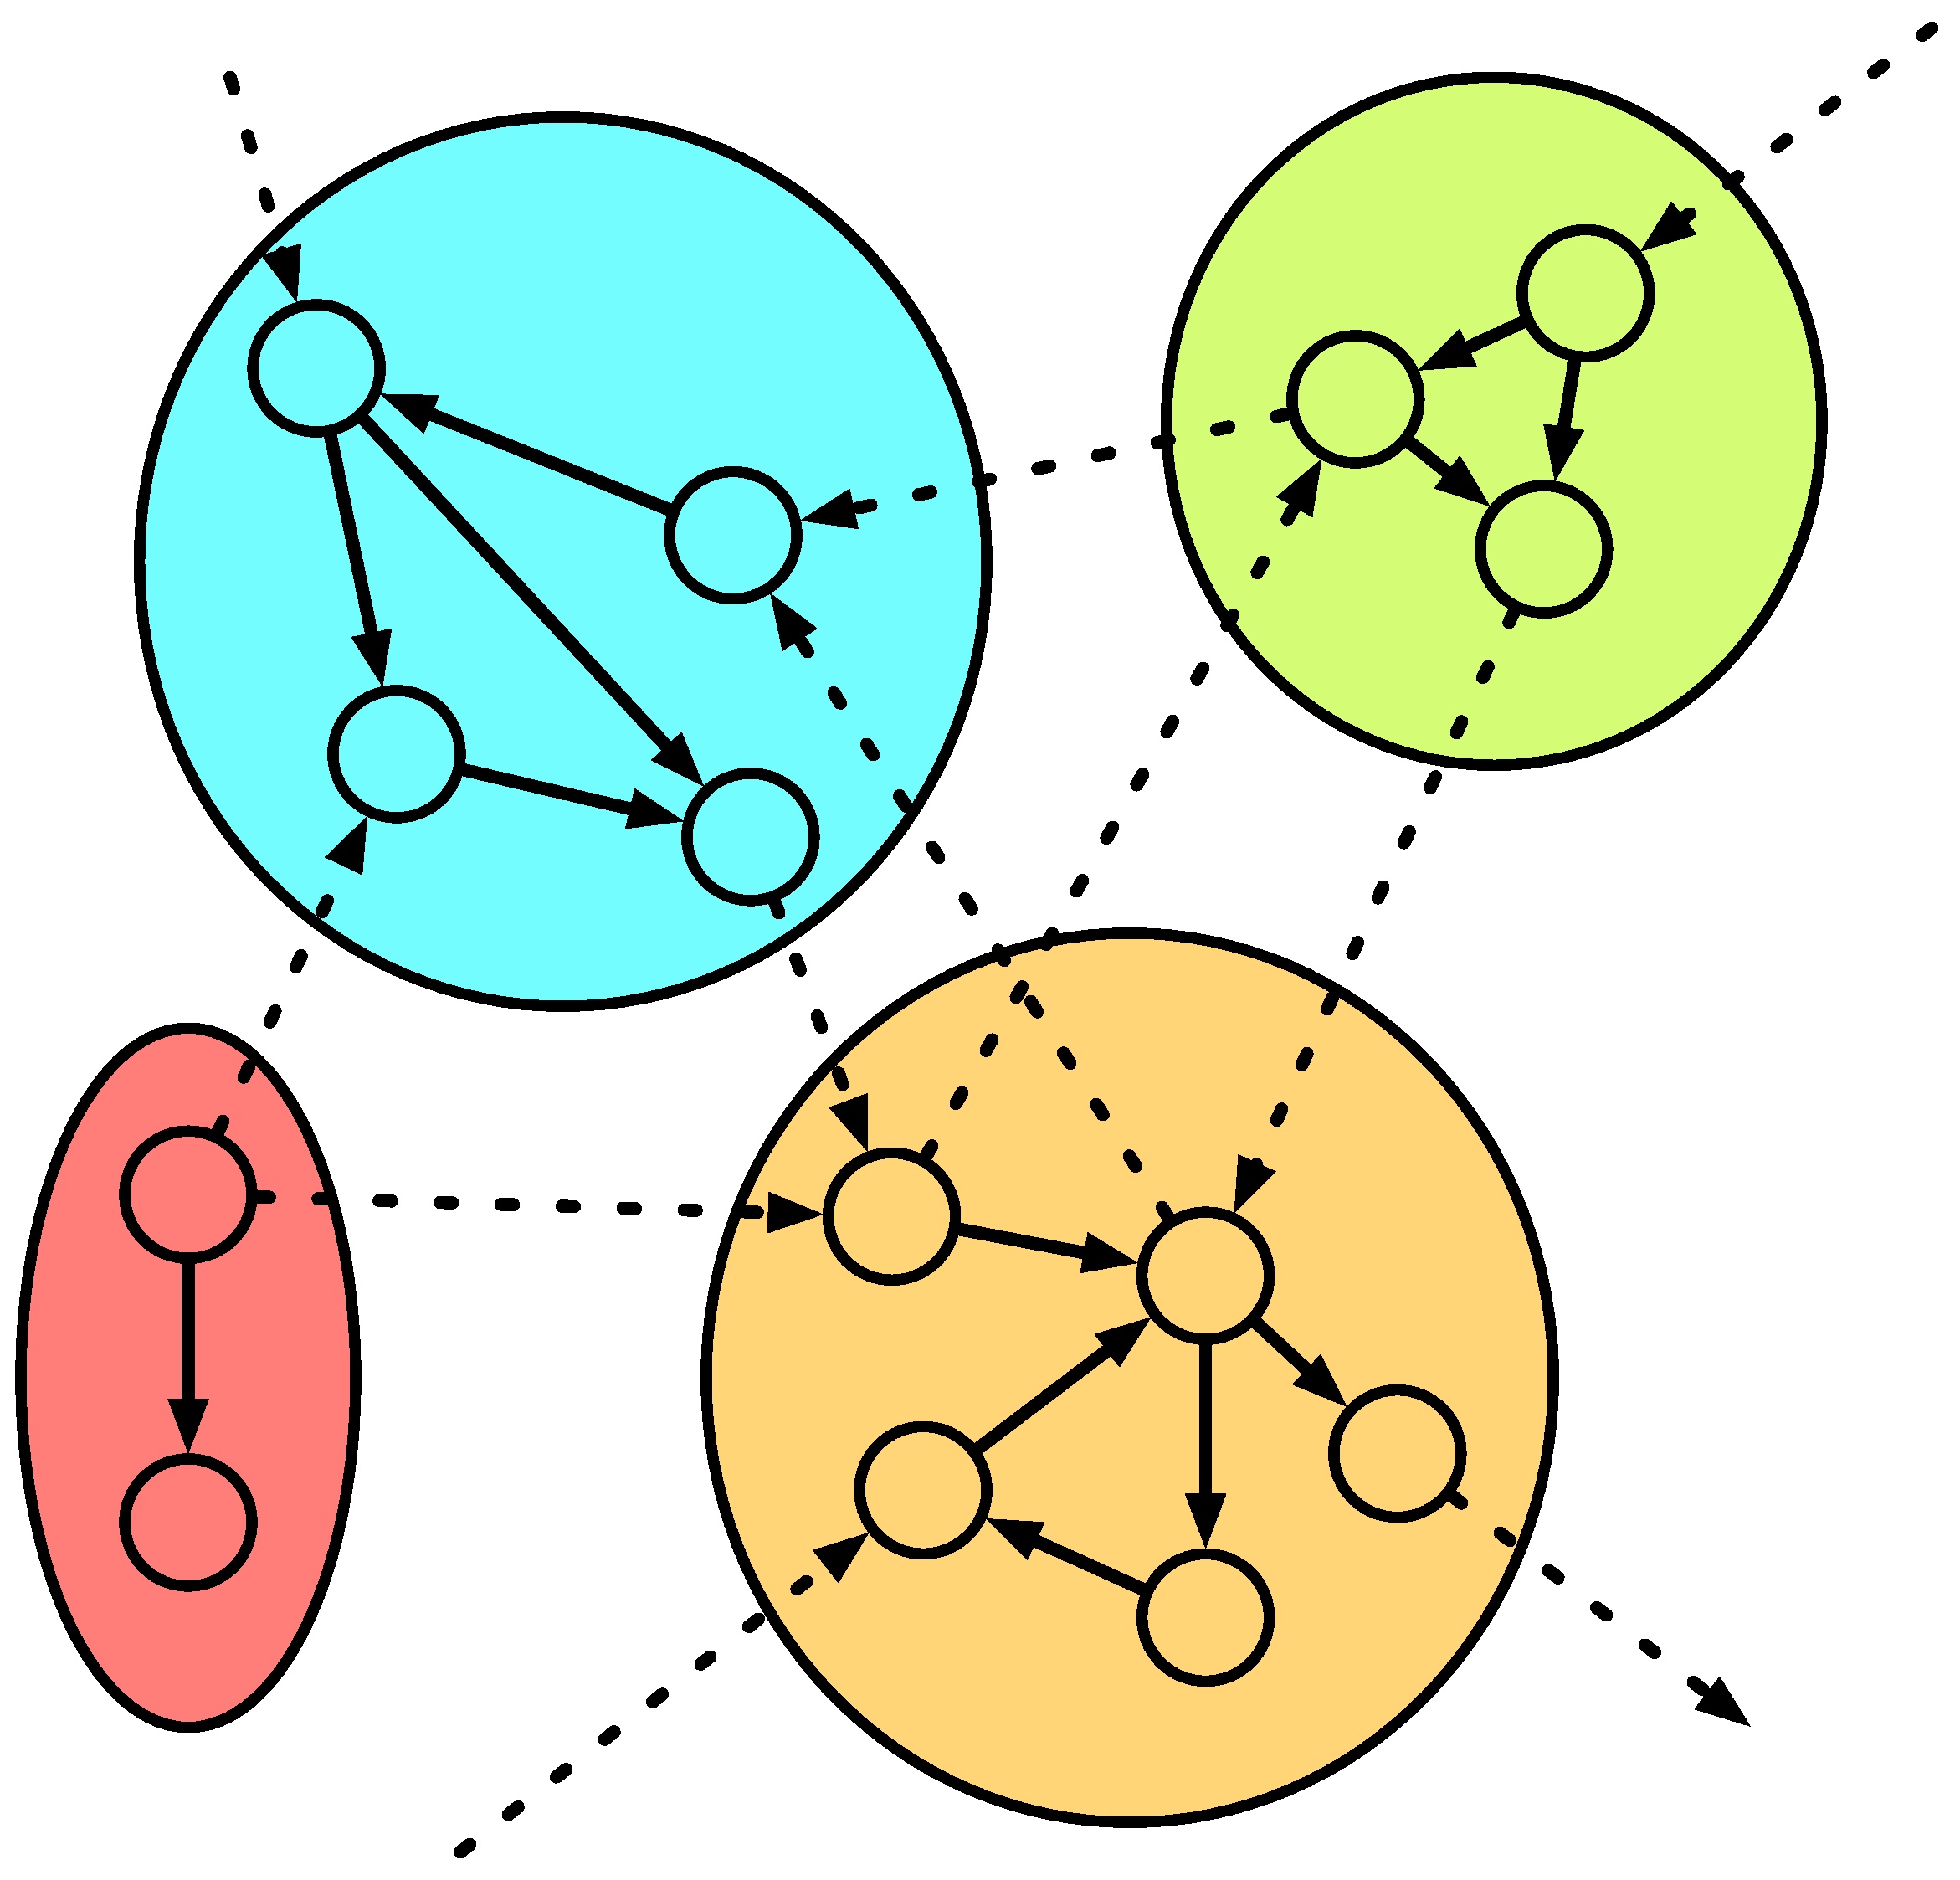
\includegraphics[width=0.50\textwidth]{Figures/Communities.eps}
\caption{Lorem ipsum.}
\label{Fig-Toy_Communities}
\end{figure}

\subsubsection{Coupled Bernoulli Process}

Lorem ipsum. \cite{ver2012information}

\begin{align}
	P(X(t, v) = 1 | \mathbf{X}(t-1), \mathbf{X}(t-2), \ldots) &= P(X(t,v) = 1 | \{ X(t-1, u) : u \in \mathcal{N}(v)\})\\
	&=\min \left\{p_{v} + \sum_{u \in \mathcal{N}(v)} \iota_{uv} 1[X(t-1, u) = 1], 1\right\}
\end{align}

\begin{figure}[h!]
  \centering
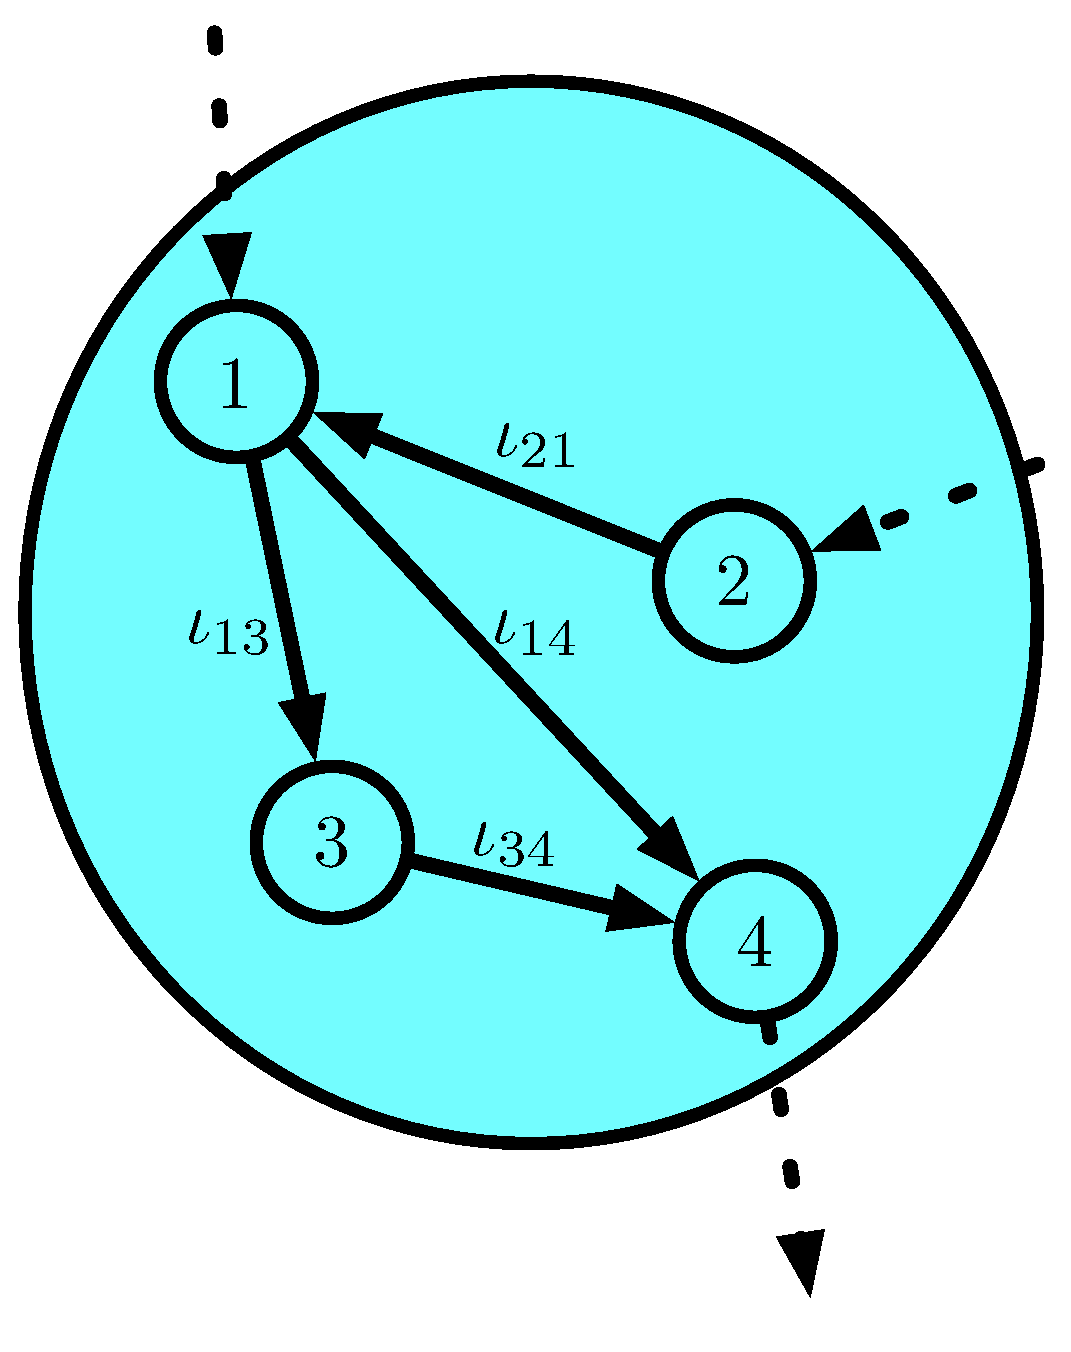
\includegraphics[width=0.3\textwidth]{Figures/Toy1.eps} \hspace{1 in}
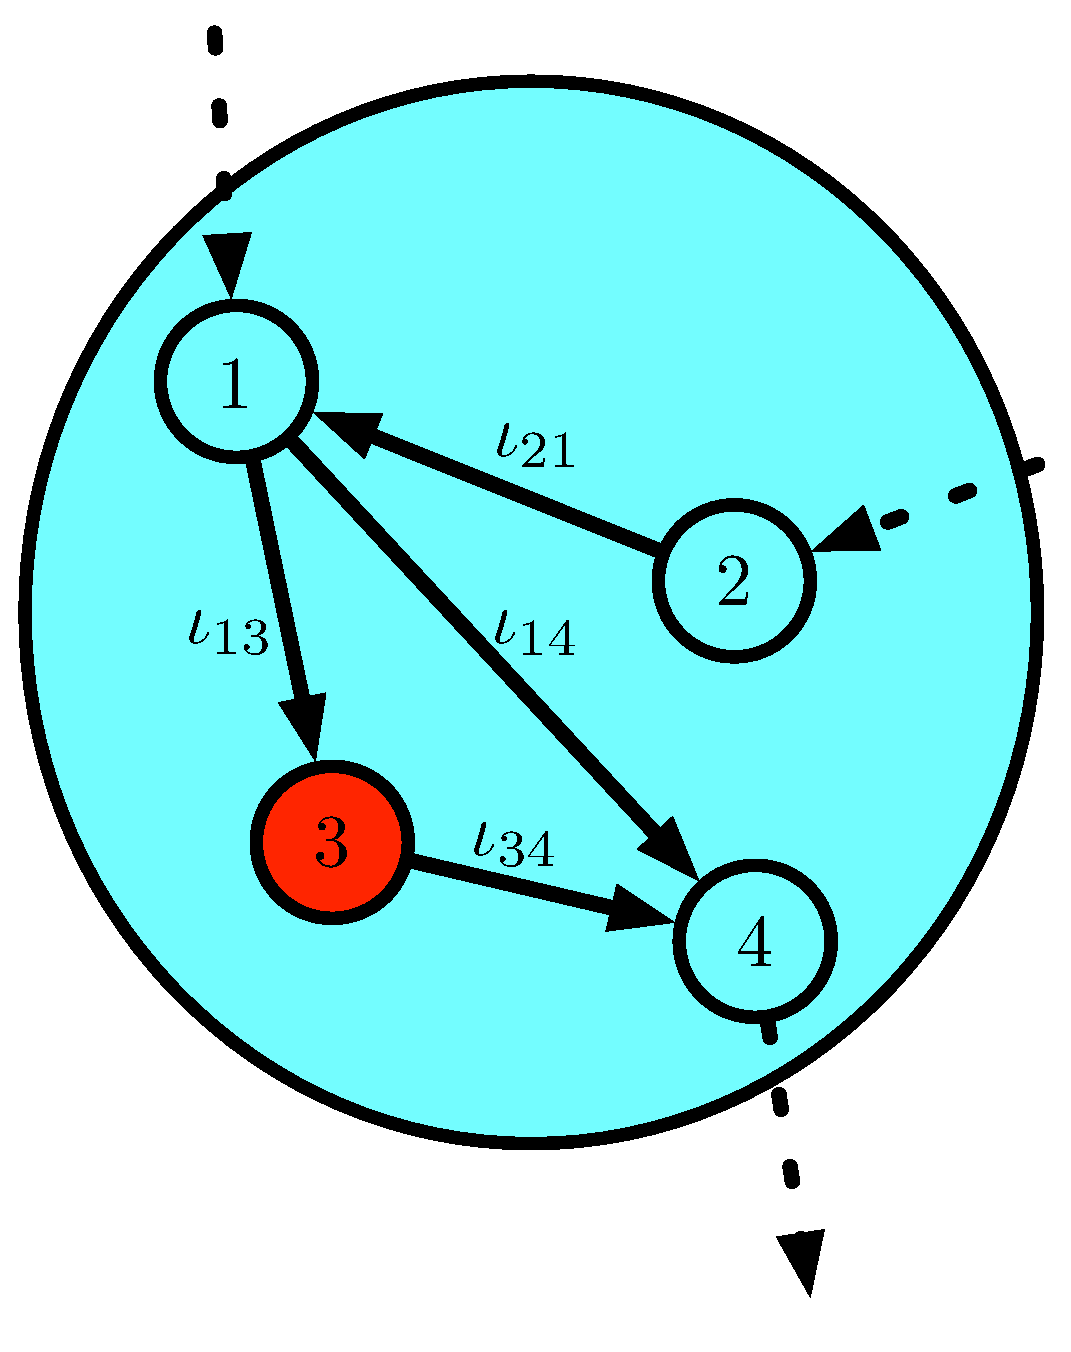
\includegraphics[width=0.3\textwidth]{Figures/Toy2.eps}
\caption{Lorem ipsum.}
\label{Fig-Toy_Bernoulli}
\end{figure}

\begin{align}
	P(X(t, 3) = 1 | \mathbf{X}(t-1), \ldots) &= P(X(t,3) = 1 | X(t, 1)) \\
		&= \min \left\{p_{3} + \iota_{13} 1[X(t-1, 1) = 1], 1\right\}\\
		&= \text{ base rate } + \text{ influence }
\end{align}

\subsection{Twitter Dataset}

\textbf{Description of the 15K dataset goes here.}

For each user $u$, we consider only the relative times of their tweets with respect to a reference time. Denote these times by $\{ \tau^{u}_{j}\}_{j = 1}^{n_{u}}$. Let the reference start time be $t_{0}$ and the coarsening amount be $\Delta t$. From the tweet times, we can generate a binary time series $\{ X(i, u)\}_{i = 1}^{T}$, where
\begin{align}
	X(i, u) = \left\{ \begin{array}{cl}
		1 &: \text{$ \exists \tau^{u}_{j} \in [t_{0} + (i - 1) \Delta t, t_{0} + i \Delta t)$} \\
		0 &: \text{ otherwise}
	\end{array}\right. .
\end{align}
In words, $X(i, u)$ is 1 if user $u$ tweeted at least once in the time interval $[t_{0} + (i - 1) \Delta t, t_{0} + i \Delta t)$, and 0 otherwise. Because the recorded time of tweets is restricted to a 1-second resolution, a natural choice for $\Delta t$ is 1 second. However, computing mutual information between second-resolution tweet series would neglect medium- to long-range influences between individuals. Thus, we generally take $\Delta t$ to be on the order of minutes.

\bibliographystyle{plain}
\bibliography{../references}

\end{document}